%%%%%%
% $Beschreibung: Heckblende $
% $Autor: ter Veen $
% $Datum: 15.06.2024 $
% $Version: 1 $
% $Pfad: SchrittmotorArduino/Manual/Tikz/Frontblende.tex $
%
%%%%%%
	
		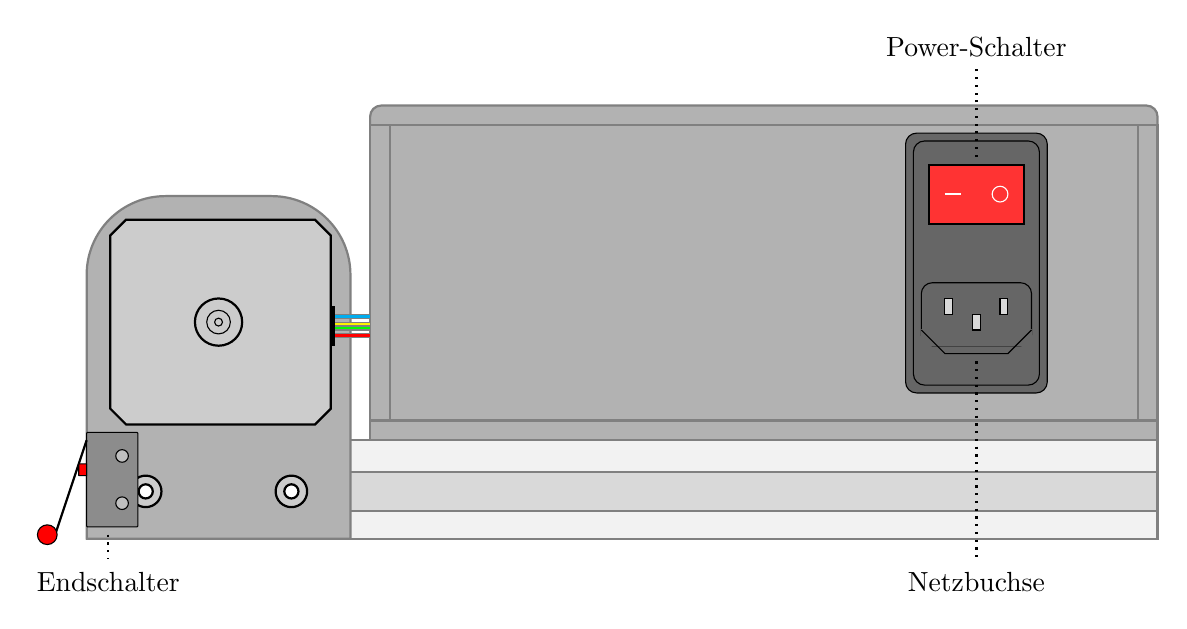
\begin{tikzpicture}
		% Gehäusedeckel
		\draw[gray, thick, fill=gray!60, rounded corners] (2,6) rectangle (12,7.25);
		
		% Gehäusemantel
		\draw[gray, thick, fill=gray!60] (2,3) rectangle (12,7);
		\draw[gray, thick, fill=gray!60] (2,3.25) rectangle (2.25,7);
		\draw[gray, thick, fill=gray!60] (11.75,3.25) rectangle (12,7);
		
		% Gehäuseboden
		\draw[gray, thick, fill=gray!60] (2,3) rectangle (12,3.25);
		
		% Alu-Profil
		\draw[gray, thick, fill=gray!10] (-1.6,1.75) rectangle (12,3);
		\draw[gray, thick, fill=gray!30] (-1.6,2.1) rectangle (12,2.6);
		
		%%% Gruppe Halterung	
		% Halterung
		\draw[gray, thick, fill=gray!60] 
		(-1.6,1.75) -- (-1.6,5.1) arc[start angle=180, end angle=90, radius=1cm] -- (0.75,6.1) arc[start angle=90, end angle=0, radius=1cm] -- (1.75,1.75) -- 
		cycle;
		
		% Motor
		\draw[black, thick, fill=gray!40]
		(-1.1,3.2) -- (-1.3,3.4) -- (-1.3,5.6) -- (-1.1,5.8) -- 
		(1.3,5.8) -- (1.5,5.6) -- (1.5,3.4) -- (1.3,3.2) -- cycle;
		% Verdrahtung
		\draw [gray, thin,fill=cyan](1.5,4.55) rectangle (2,4.6); % blau
		\draw [gray, thin,fill=yellow](1.5,4.45) rectangle (2,4.5); % gelb
		\draw [gray, thin,fill=green](1.5,4.4) rectangle (2,4.45); % grün
		\draw [gray, thin,fill=red](1.5,4.35) rectangle (2,4.3); % rot
		\draw [black, thin,fill=black](1.5,4.2) rectangle (1.55,4.7); % buchse
		
		% Lagerung Zahnrad
		\draw[black, thick, fill=gray!40] (0.075,4.5) circle (0.3);
		\draw[black, thin, fill=gray!40] (0.075,4.5) circle (0.15);
		\draw[black, thin, fill=gray!40] (0.075,4.5) circle (0.05);
		
		% Befestigungsschraube 1
		\draw[black, thick, fill=gray!40] (1,2.35) circle (0.2);
		\draw[black, thick, fill=white] (1,2.35) circle (0.09);
		% Befestigungsschraube 2
		\draw[black, thick, fill=gray!40] (-0.85,2.35) circle (0.2);
		\draw[black, thick, fill=white] (-0.85,2.35) circle (0.09);
		
		% Endschalter
		\draw[black, thin, fill=gray!90, rounded corners=0.3] (-1.6,1.9) rectangle (-0.95,3.1);
		\draw[black, thick](-1.6,3) -- (-2,1.8);
		\draw[black, thin, fill=red, rounded corners=0.1] (-1.6, 2.7) rectangle (-1.7,2.55);
		\draw [black, thin, fill=red] (-2.1,1.8) circle (0.125);
		\draw [black, thin, fill=gray!50] (-1.15,2.2) circle (0.08);
		\draw [black, thin, fill=gray!50] (-1.15,2.8) circle (0.08);
		%%%
		
		% Netzbuchse
		\draw[black, thin, fill=black!60, rounded corners] (8.8,3.6) rectangle (10.6,6.9);
		\draw[black, thin, fill=black!60, rounded corners] (8.9,3.7) rectangle (10.5,6.8);
		% Schalter
		\draw[black, thick, fill=red!80] (9.1,5.75) rectangle (10.3,6.5);
		\draw[white, thick] (9.3,6.125) -- (9.5,6.125); % Ein
		\draw[white, thin] (10,6.125) circle  (0.1); % Aus
		% Buchse
		\draw[black, thin, rounded corners] (9,4.2) rectangle (10.4,5);
		\draw[black!60, thin, fill=black!60] (9,4.2) rectangle (10.4,4.4);
		\draw [black] (9,4.4) -- (9.3,4.1) -- (10.1,4.1) -- (10.4,4.4);
		% Pins
		\draw[black, thin, fill=gray!30] (9.3,4.6) rectangle (9.4,4.8);
		\draw[black, thin, fill=gray!30] (10,4.6) rectangle (10.1,4.8);
		\draw[black, thin, fill=gray!30] (9.65,4.4) rectangle (9.75,4.6);
		
		% Punkt-Linien für Labels
		\draw[dotted, thick] (9.7,6.6) -- (9.7,7.75); % Power-Schalter
		\draw[dotted, thick] (9.7,4) -- (9.7,1.5); % Netzbuchse
		\draw[dotted, thick] (-1.325,1.8) -- (-1.325,1.5); % Endschalter
		
		% Labels
		\node[] at (9.7,8) {Power-Schalter};
		\node[] at (9.7,1.2) {Netzbuchse};
		\node[] at (-1.325,1.2) {Endschalter};
		
	\end{tikzpicture}